\makesection{Conclusion}

\begin{frame}{Conclusion}

    \begin{itemize}
        \item Achievements:
        \begin{multicols}{4}
            \begin{tcolorbox}[colback=boxcolor, colframe=boxcolor, width=0.235\textwidth, height=4.5cm, rounded corners]
                \centering
                Modular and maintainable architecture and optimized codebase.
            \end{tcolorbox}
            
            \begin{tcolorbox}[colback=boxcolor, colframe=boxcolor, width=0.235\textwidth, height=4.5cm, rounded corners]
                \centering
                Design of a customizable physics engine which supports convex polygons.
            \end{tcolorbox}
            
            \begin{tcolorbox}[colback=boxcolor, colframe=boxcolor, width=0.235\textwidth, height=4.5cm, rounded corners]
                \centering
                Framework (based on OOP) that can be readily extended.
            \end{tcolorbox}
            
            \begin{tcolorbox}[colback=boxcolor, colframe=boxcolor, width=0.235\textwidth, height=4.5cm, rounded corners]
                \centering
                Enhanced user experience with new features (terrain, items, graphics..)
            \end{tcolorbox}
        \end{multicols}
        \item Tradeoff: OOP architecture is less performant than flecs.
    \end{itemize}
\end{frame}

\begin{frame}{Comparision of the Game Versions}
    \begin{minipage}{\textwidth}
        \centering
        \begin{minipage}{.495\textwidth}
            \begin{figure}
                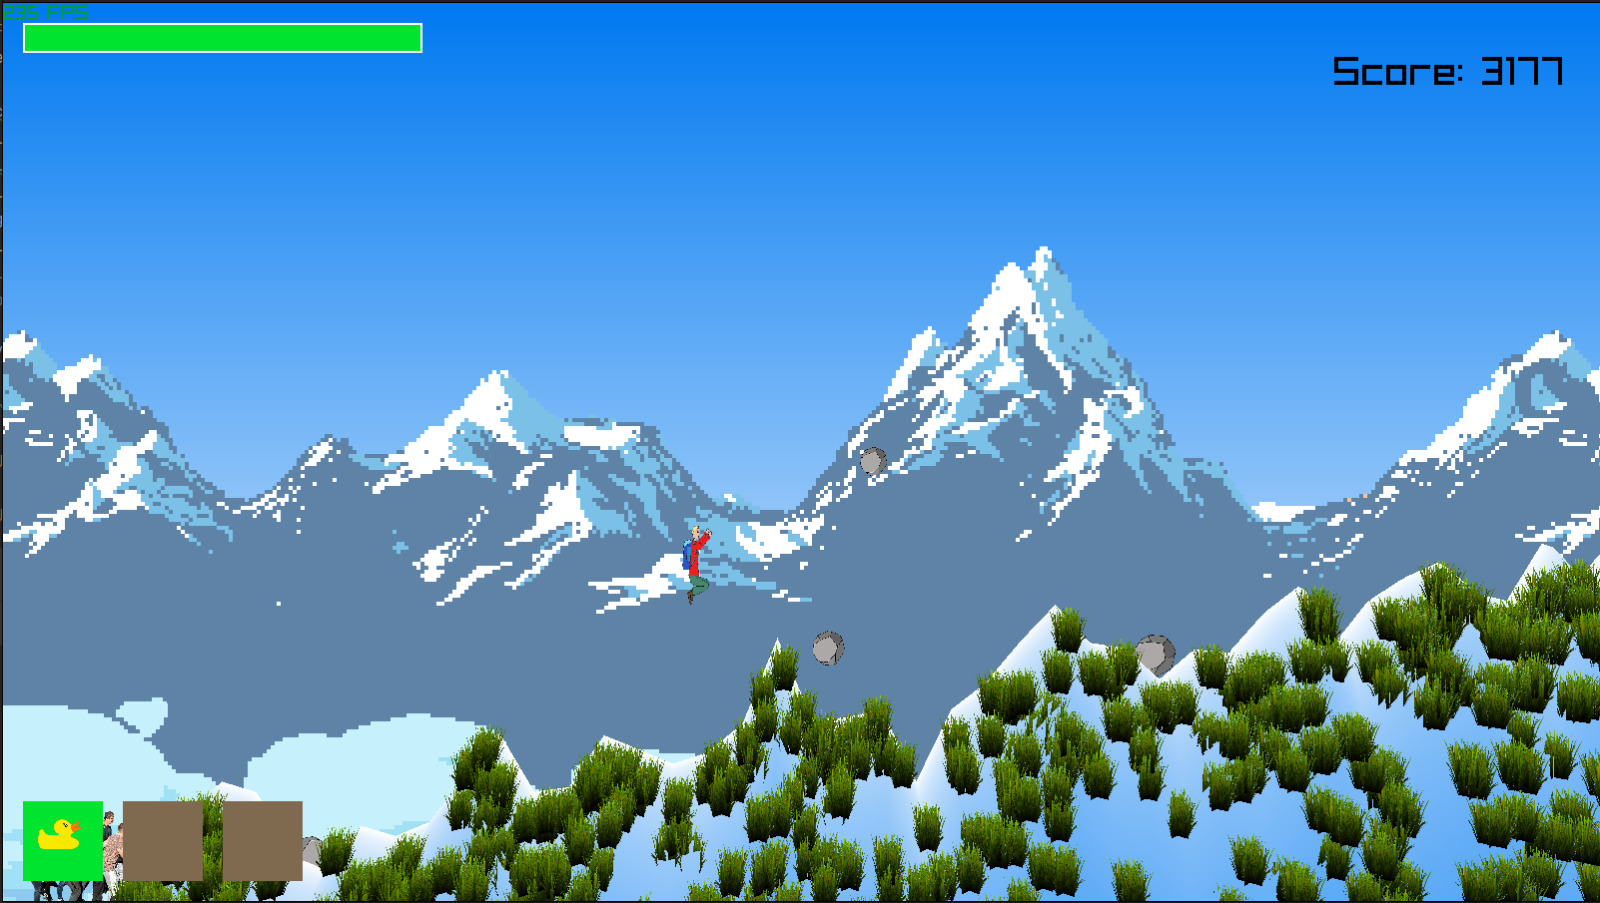
\includegraphics[width=\textwidth]{../figures/old_game.jpeg}
                    \caption{Ferienakademie 2023\phantom{y}}
            \end{figure}

        \end{minipage}
        \begin{minipage}{.495\textwidth}

                \begin{figure}
                    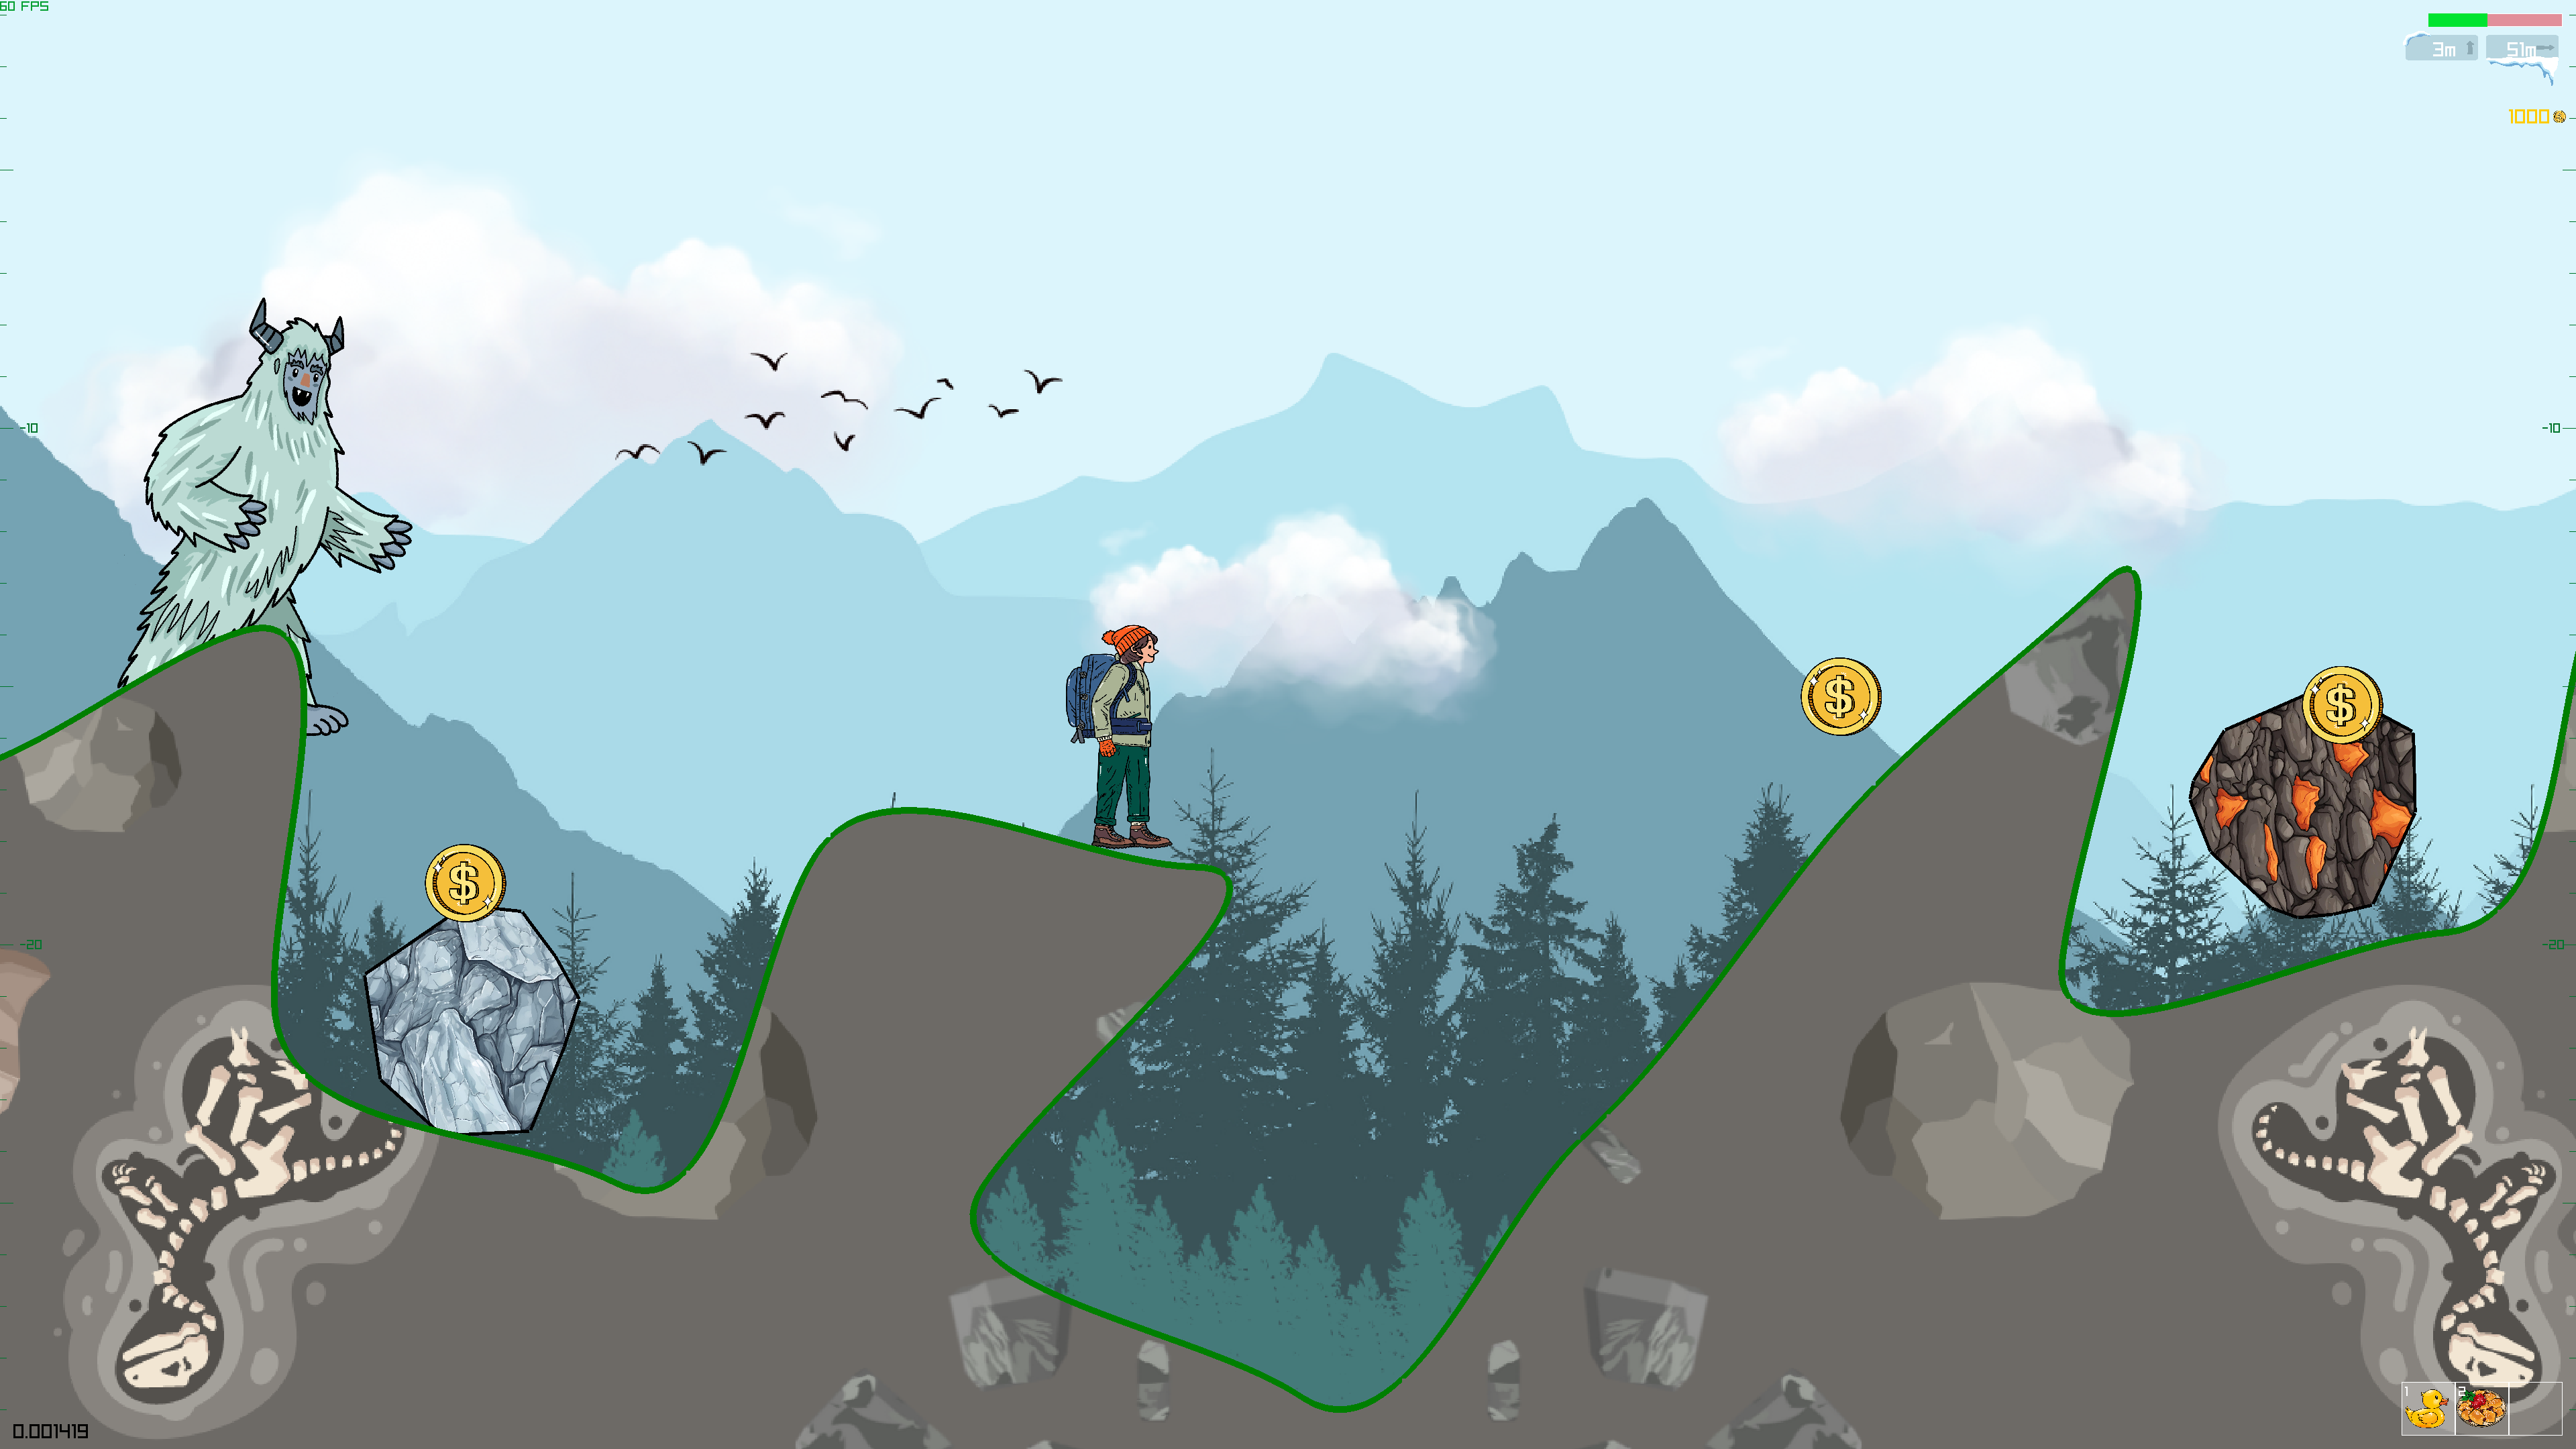
\includegraphics[width=\textwidth]{../figures/new_game.png}
                    \caption{Today}
                \end{figure}

        \end{minipage}
    \end{minipage}
    %\vspace{-.45cm}
\end{frame}

\begin{frame}{Comparison of the Game Versions}
    \centering
    \begin{tabular}{cc}
        \begin{tcolorbox}[colback=boxcolor, width=0.5\textwidth, height=6.5cm, colframe=boxcolor, rounded corners]
            \textbf{Ferienakademie 2023}
            \begin{itemize}
                \setbeamertemplate{itemize item}{\textcolor{red}{\textbf{-}}}
                \item not all items have a functionality
                \item ``buggy'' physics, dependent on fps
                \item linear terrain
                \item based on Entity-Component-System
                \item[\textcolor{green}{\textbf{+}}] good performance
                \item[\textcolor{green}{\textbf{+}}] great ideas!
            \end{itemize}
        \end{tcolorbox}
        &
        \begin{tcolorbox}[colback=boxcolor, width=0.5\textwidth, height=6.5cm, colframe=boxcolor, rounded corners]
            \textbf{New "Surviving Sarntal"}
            \begin{itemize}
                \setbeamertemplate{itemize item}{\textcolor{green}{\textbf{+}}}
                \item unique items
                \item accurate physics, independent of fps
                \item spline-based terrain with overhangs
                \item increasing difficulty
                \item new audio and visuals 
                \item modular and maintainable code based on OOP
                \item addition of game menu
            \end{itemize}
        \end{tcolorbox}
    \end{tabular}
\end{frame}

\begin{frame}{Future Work}
    \begin{itemize}
        \item Multiplayer modes and leaderboard integration.
        \item New game items and biomes.
        \item Difficulty settings, coin shop to buy upgrades
        \item Further enhancements to the physics engine:
        \begin{itemize}
            \item Improved performance with parallel batch processing and spatial data structures.
            \item Friction and air resistance.
            \item Reduction of jitter.
        \end{itemize}
    \end{itemize}
    \centering
    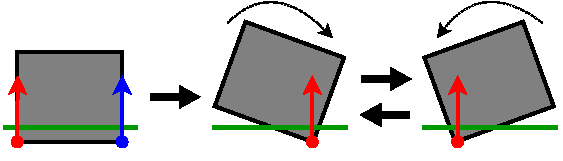
\includegraphics[width = .5\textwidth]{../figures/physics/jitter.pdf}
\end{frame}